% Options for packages loaded elsewhere
\PassOptionsToPackage{unicode}{hyperref}
\PassOptionsToPackage{hyphens}{url}
\documentclass[
  ignorenonframetext,
  aspectratio=169]{beamer}
\newif\ifbibliography
\usepackage{pgfpages}
\setbeamertemplate{caption}[numbered]
\setbeamertemplate{caption label separator}{: }
\setbeamercolor{caption name}{fg=normal text.fg}
\beamertemplatenavigationsymbolsempty
% remove section numbering
\setbeamertemplate{part page}{
  \centering
  \begin{beamercolorbox}[sep=16pt,center]{part title}
    \usebeamerfont{part title}\insertpart\par
  \end{beamercolorbox}
}
\setbeamertemplate{section page}{
  \centering
  \begin{beamercolorbox}[sep=12pt,center]{section title}
    \usebeamerfont{section title}\insertsection\par
  \end{beamercolorbox}
}
\setbeamertemplate{subsection page}{
  \centering
  \begin{beamercolorbox}[sep=8pt,center]{subsection title}
    \usebeamerfont{subsection title}\insertsubsection\par
  \end{beamercolorbox}
}
% Prevent slide breaks in the middle of a paragraph
\widowpenalties 1 10000
\raggedbottom
\AtBeginPart{
  \frame{\partpage}
}
\AtBeginSection{
  \ifbibliography
  \else
    \frame{\sectionpage}
  \fi
}
\AtBeginSubsection{
  \frame{\subsectionpage}
}
\usepackage{iftex}
\ifPDFTeX
  \usepackage[T1]{fontenc}
  \usepackage[utf8]{inputenc}
  \usepackage{textcomp} % provide euro and other symbols
\else % if luatex or xetex
  \usepackage{unicode-math} % this also loads fontspec
  \defaultfontfeatures{Scale=MatchLowercase}
  \defaultfontfeatures[\rmfamily]{Ligatures=TeX,Scale=1}
\fi
\usepackage{lmodern}
\ifPDFTeX\else
  % xetex/luatex font selection
\fi
% Use upquote if available, for straight quotes in verbatim environments
\IfFileExists{upquote.sty}{\usepackage{upquote}}{}
\IfFileExists{microtype.sty}{% use microtype if available
  \usepackage[]{microtype}
  \UseMicrotypeSet[protrusion]{basicmath} % disable protrusion for tt fonts
}{}
\makeatletter
\@ifundefined{KOMAClassName}{% if non-KOMA class
  \IfFileExists{parskip.sty}{%
    \usepackage{parskip}
  }{% else
    \setlength{\parindent}{0pt}
    \setlength{\parskip}{6pt plus 2pt minus 1pt}}
}{% if KOMA class
  \KOMAoptions{parskip=half}}
\makeatother
% definitions for citeproc citations
\NewDocumentCommand\citeproctext{}{}
\NewDocumentCommand\citeproc{mm}{%
  \begingroup\def\citeproctext{#2}\cite{#1}\endgroup}
\makeatletter
 % allow citations to break across lines
 \let\@cite@ofmt\@firstofone
 % avoid brackets around text for \cite:
 \def\@biblabel#1{}
 \def\@cite#1#2{{#1\if@tempswa , #2\fi}}
\makeatother
\newlength{\cslhangindent}
\setlength{\cslhangindent}{1.5em}
\newlength{\csllabelwidth}
\setlength{\csllabelwidth}{3em}
\newenvironment{CSLReferences}[2] % #1 hanging-indent, #2 entry-spacing
 {\begin{list}{}{%
  \setlength{\itemindent}{0pt}
  \setlength{\leftmargin}{0pt}
  \setlength{\parsep}{0pt}
  % turn on hanging indent if param 1 is 1
  \ifodd #1
   \setlength{\leftmargin}{\cslhangindent}
   \setlength{\itemindent}{-1\cslhangindent}
  \fi
  % set entry spacing
  \setlength{\itemsep}{#2\baselineskip}}}
 {\end{list}}
\usepackage{calc}
\newcommand{\CSLBlock}[1]{\hfill\break\parbox[t]{\linewidth}{\strut\ignorespaces#1\strut}}
\newcommand{\CSLLeftMargin}[1]{\parbox[t]{\csllabelwidth}{\strut#1\strut}}
\newcommand{\CSLRightInline}[1]{\parbox[t]{\linewidth - \csllabelwidth}{\strut#1\strut}}
\newcommand{\CSLIndent}[1]{\hspace{\cslhangindent}#1}
\setlength{\emergencystretch}{3em} % prevent overfull lines
\providecommand{\tightlist}{%
  \setlength{\itemsep}{0pt}\setlength{\parskip}{0pt}}
% ============================================================
%  beamer_preamble.tex
%  Executive deck — Indonesia CVD / FAIR Choices analysis
%  World Bank  ·  University of Washington collaboration
%  (Adapted in-repo from the prior project preamble: default Beamer
%   look, Calibri fonts, colored blocks + scenario palette, then
%   rebranded for the World Bank – UW Indonesia CVD work.)
% ============================================================

% ── Beamer theme (clean default look, lightly branded) ───────────────────────
\usetheme{default}
\usecolortheme{default}
\usefonttheme{professionalfonts}

% ── XeLaTeX fonts (requires xelatex engine) ─────────────────────────────────
\usepackage{fontspec}
\setmainfont{Calibri}[
  BoldFont       = Calibri Bold,
  ItalicFont     = Calibri Italic,
  BoldItalicFont = Calibri Bold Italic
]
\setsansfont{Calibri}
\setmonofont{Consolas}

% ── Packages ────────────────────────────────────────────────────────────────
\usepackage{booktabs}
\usepackage{xcolor}
\usepackage{colortbl}
\usepackage{array}
\usepackage{graphicx}
\usepackage{ragged2e}
\usepackage{microtype}
\usepackage{tabularx}
\usepackage{makecell}
\usepackage{multirow}
\usepackage{tikz}
\usetikzlibrary{arrows.meta, positioning, shapes.geometric, calc, backgrounds, fit}
\usepackage{hyperref}

% ── Project colour palette (World Bank – UW; colour-blind aware) ─────────────
\definecolor{wbnavy}{HTML}{0F2A56}        % primary dark navy (World Bank)
\definecolor{wbblue}{HTML}{2166AC}        % accent blue
\definecolor{uwpurple}{HTML}{4B2E83}      % UW brand purple (secondary accent)
\definecolor{uwgold}{HTML}{B7A57A}        % UW gold (rare accent)

% Scenario-family colours (must match ggplot palette in the .Rmd)
\definecolor{clinicalcol}{HTML}{3B6FB6}   % clinical scenarios (blue)
\definecolor{phcol}{HTML}{1B9E77}         % public-health scenarios (teal-green)
\definecolor{combinedcol}{HTML}{08306B}   % combined package (dark navy)
\definecolor{comparatorgrey}{HTML}{9E9E9E}% comparators / baseline context
\definecolor{incidencecol}{HTML}{2166AC}  % incidence (Well->Sick) effects
\definecolor{casefatalcol}{HTML}{B2182B}  % case-fatality (Sick->Death) effects
\definecolor{bgmortcol}{HTML}{7F7F7F}     % background mortality
\definecolor{highlightblue}{HTML}{DBEAFE} % table row highlight
\definecolor{highlightgold}{HTML}{FCEFCB} % combined-package row highlight

% ── Light branding: navy frame titles, blue structure accents ───────────────
\setbeamercolor{structure}{fg=wbblue}
\setbeamercolor{title}{fg=wbnavy}
\setbeamercolor{subtitle}{fg=wbblue}
\setbeamercolor{author}{fg=black}
\setbeamercolor{date}{fg=black}
\setbeamercolor{institute}{fg=black}
\setbeamercolor{frametitle}{fg=wbnavy}
\setbeamercolor{normal text}{fg=black}
\setbeamerfont{frametitle}{series=\bfseries}
\setbeamerfont{title}{series=\bfseries}

% Keep default background/frametitle templates (clean, no heavy canvas).

% ── Colored blocks (boxes) ──────────────────────────────────────────────────
\setbeamercolor{block title}{bg=wbnavy!12, fg=wbnavy}
\setbeamercolor{block body}{bg=wbnavy!5}

\setbeamercolor{block title alerted}{bg=casefatalcol!15, fg=casefatalcol!80!black}
\setbeamercolor{block body alerted}{bg=casefatalcol!6}

\setbeamercolor{block title example}{bg=phcol!15, fg=phcol!75!black}
\setbeamercolor{block body example}{bg=phcol!6}

% Custom family-coloured blocks
\newenvironment{clinicalblock}[1]{%
  \setbeamercolor{block title}{bg=clinicalcol!16, fg=clinicalcol!80!black}%
  \setbeamercolor{block body}{bg=clinicalcol!6}%
  \begin{block}{#1}%
}{\end{block}}

\newenvironment{phblock}[1]{%
  \setbeamercolor{block title}{bg=phcol!16, fg=phcol!75!black}%
  \setbeamercolor{block body}{bg=phcol!6}%
  \begin{block}{#1}%
}{\end{block}}

\newenvironment{combinedblock}[1]{%
  \setbeamercolor{block title}{bg=combinedcol!18, fg=combinedcol}%
  \setbeamercolor{block body}{bg=combinedcol!7}%
  \begin{block}{#1}%
}{\end{block}}

% ── Bullet style (blue accent) ──────────────────────────────────────────────
\setbeamertemplate{itemize item}{\textcolor{wbblue}{\textbullet}}
\setbeamertemplate{itemize subitem}{\textcolor{wbblue}{--}}
\setbeamertemplate{itemize subsubitem}{\textcolor{wbblue}{\textperiodcentered}}
\setbeamertemplate{enumerate item}{\textcolor{wbblue}{\insertenumlabel.}}

% ── Headline highlight command ──────────────────────────────────────────────
\newcommand{\hlkey}[1]{%
  \colorbox{highlightblue}{\textcolor{wbnavy}{\textbf{#1}}}%
}

% ── Clean footer (World Bank – UW) ──────────────────────────────────────────
\setbeamertemplate{footline}{%
  \leavevmode
  \hbox{%
    \begin{beamercolorbox}[wd=0.34\paperwidth, ht=2.25ex, dp=1ex, left]{author in head/foot}%
      \hspace{1em}\usebeamerfont{author in head/foot}%
      \textcolor{black!60}{\footnotesize World Bank \textperiodcentered\ University of Washington}%
    \end{beamercolorbox}%
    \begin{beamercolorbox}[wd=0.56\paperwidth, ht=2.25ex, dp=1ex, center]{title in head/foot}%
      \usebeamerfont{title in head/foot}%
      \textcolor{black!60}{\footnotesize Indonesia CVD --- Health Impact, Costs \& Economic Returns}%
    \end{beamercolorbox}%
    \begin{beamercolorbox}[wd=0.10\paperwidth, ht=2.25ex, dp=1ex, right]{date in head/foot}%
      \usebeamerfont{date in head/foot}%
      \textcolor{black!60}{\footnotesize \insertframenumber{}/\inserttotalframenumber}%
      \hspace{0.5em}%
    \end{beamercolorbox}%
  }%
  \vskip0pt%
}
\setbeamertemplate{navigation symbols}{}

% ── Section divider slides (auto from # headers) ────────────────────────────
\AtBeginSection[]{%
  \begin{frame}
    \vfill
    \centering
    \begin{beamercolorbox}[sep=10pt, center, shadow=false, rounded=true]{block title}
      \usebeamerfont{title}\insertsectionhead\par
    \end{beamercolorbox}
    \vfill
  \end{frame}
}
\usepackage{booktabs}
\usepackage{longtable}
\usepackage{array}
\usepackage{multirow}
\usepackage{wrapfig}
\usepackage{float}
\usepackage{colortbl}
\usepackage{pdflscape}
\usepackage{tabu}
\usepackage{threeparttable}
\usepackage{threeparttablex}
\usepackage[normalem]{ulem}
\usepackage{makecell}
\usepackage{xcolor}
\usepackage{bookmark}
\IfFileExists{xurl.sty}{\usepackage{xurl}}{} % add URL line breaks if available
\urlstyle{same}
\hypersetup{
  pdftitle={Reducing Cardiovascular Disease in Indonesia},
  pdfauthor={World Bank \textbackslash cdot University of Washington},
  hidelinks,
  pdfcreator={LaTeX via pandoc}}

\title{Reducing Cardiovascular Disease in Indonesia}
\subtitle{Health Impact, Costs, and Economic Returns of Clinical and
Public-Health Interventions, 2025--2050}
\author{World Bank \(\cdot\) University of Washington}
\date{August 2026}
\institute{Briefing for the Ministry of Health, Republic of Indonesia}

\begin{document}
\frame{\titlepage}

\section{Reducing CVD in Indonesia}\label{reducing-cvd-in-indonesia}

\begin{frame}{Why this matters for Indonesia}
\phantomsection\label{why-this-matters-for-indonesia}
\begin{columns}[T]
\begin{column}{0.52\textwidth}
\begin{block}{Cardiovascular disease is Indonesia's largest health burden}
\normalsize
Under current trends, a person reaching age 30 faces roughly a
\hlkey{14.5\% chance} of dying from cardiovascular disease
before age 70 --- the CVD ``40q30''. Most of this is \textbf{preventable or treatable}.
\end{block}
\end{column}
\begin{column}{0.46\textwidth}
\begin{itemize}\itemsep4pt
  \item Premature CVD deaths (ages 30--69) have risen for two decades and remain high.
  \item Two complementary levers:
  \begin{itemize}
    \item \textcolor{clinicalcol}{\textbf{Clinical care}} --- prevent and better treat established disease.
    \item \textcolor{phcol}{\textbf{Population prevention}} --- tobacco, salt, trans-fat, sugary drinks, alcohol.
  \end{itemize}
  \item This analysis weighs their \textbf{health impact, cost, and economic return} together.
\end{itemize}
\end{column}
\end{columns}

\vspace{3pt}

\footnotesize Source: Indonesia CVD model (calibrated to GBD 2023; UN
World Population Prospects 2024). CVD 40q30 = probability of dying from
cardiovascular disease between exact ages 30 and 70.
\end{frame}

\begin{frame}{What this analysis set out to do}
\phantomsection\label{what-this-analysis-set-out-to-do}
\begin{block}{General aim}
\normalsize Estimate the \textbf{health and economic effects} of scaling up evidence-based
\textbf{clinical} and \textbf{public-health} cardiovascular interventions in Indonesia through \textbf{2050}.
\end{block}

\vspace{2pt}
\begin{columns}[T]
\begin{column}{0.33\textwidth}
\begin{clinicalblock}{Aim 1 --- Burden}
\footnotesize Project the CVD burden and the premature-mortality indicator (CVD 40q30) under the \textbf{status quo} and under \textbf{alternative intervention scenarios}.
\end{clinicalblock}
\end{column}
\begin{column}{0.33\textwidth}
\begin{phblock}{Aim 2 --- Value for money}
\footnotesize Estimate \textbf{deaths averted}, mortality reductions, \textbf{incremental costs}, and \textbf{cost-effectiveness} for each intervention and package.
\end{phblock}
\end{column}
\begin{column}{0.33\textwidth}
\begin{combinedblock}{Aim 3 --- Economic return}
\footnotesize Estimate \textbf{economic benefits}, \textbf{benefit--cost ratios}, and the \textbf{added value of combining} clinical and public-health action.
\end{combinedblock}
\end{column}
\end{columns}

\vspace{3pt}

\footnotesize Horizon 2025--2050; the ``status quo'' baseline is the
no-new-intervention comparator against which every scenario is measured.
\end{frame}

\begin{frame}{Executive summary --- the headline numbers}
\phantomsection\label{executive-summary-the-headline-numbers}
\begin{columns}[T]
\begin{column}{0.5\textwidth}
\begin{combinedblock}{Combining clinical + public health is the big prize}
\footnotesize Together they could avert about \hlkey{3.5M deaths} over 2025--2050,
cut the CVD 40q30 in 2050 by \hlkey{29\%}, and return about
\hlkey{79.1 int\$} in benefits per int\$ spent.
\end{combinedblock}
\end{column}
\begin{column}{0.5\textwidth}
\begin{itemize}\footnotesize\itemsep3pt
  \item \textcolor{clinicalcol}{\textbf{All clinical interventions}}: $\approx$2.0M deaths averted; CVD 40q30 down 20\% by 2050.
  \item \textcolor{phcol}{\textbf{All public-health policies}}: $\approx$1.6M deaths averted; benefit--cost ratio $\approx$1,240.
  \item \textbf{Most impactful single levers}: \textcolor{clinicalcol}{Primary CVD prevention} and \textcolor{phcol}{Tobacco tax}.
  \item \textbf{Affordability}: the combined package costs about US\$4,814 per death averted.
\end{itemize}
\end{column}
\end{columns}

\vspace{2pt}

\scriptsize All figures from the model's cost/value workbooks. Deaths
averted are cumulative 2025--2050 across modeled cardiovascular and
diabetes causes; benefits valued per the Reference Case (Robinson 2019)
in PPP international dollars (Robinson, Hammitt, and O'Keeffe 2019).
\end{frame}

\begin{frame}{How the model works --- in plain language}
\phantomsection\label{how-the-model-works-in-plain-language}
\begin{columns}[T]
\begin{column}{0.54\textwidth}
\footnotesize
\begin{enumerate}\itemsep3pt
  \item \textbf{People \& demography.} Indonesia's population is projected by age and sex (UN World Population Prospects 2024).
  \item \textbf{Starting health.} Disease and death rates are set to Indonesia's data (GBD 2023) and calibrated to match observed levels.
  \item \textbf{Year-by-year simulation.} Each year people can develop cardiovascular disease or diabetes, survive, or die.
  \item \textbf{Interventions.} Clinical and public-health scenarios change how many people develop disease and how many survive it.
  \item \textbf{Outcomes.} The model reports deaths, healthy years (DALYs), premature-mortality (40q30), costs, cost-effectiveness, and economic returns.
\end{enumerate}
\end{column}
\begin{column}{0.44\textwidth}
\begin{block}{One consistent engine}
\footnotesize Every scenario runs through the \textbf{same} projection, so results are directly comparable and the \textbf{combined} package is modeled as one run --- not a sum of separate estimates.
\end{block}
\vspace{2pt}
\scriptsize Calibration fits the model to GBD estimates using a standard numerical optimiser (Nelder--Mead). Life expectancy for lost-years and economic value uses UN WPP 2024.
\end{column}
\end{columns}
\end{frame}

\begin{frame}{How interventions change the disease pathway}
\phantomsection\label{how-interventions-change-the-disease-pathway}
\vspace{-2pt}
\begin{center}
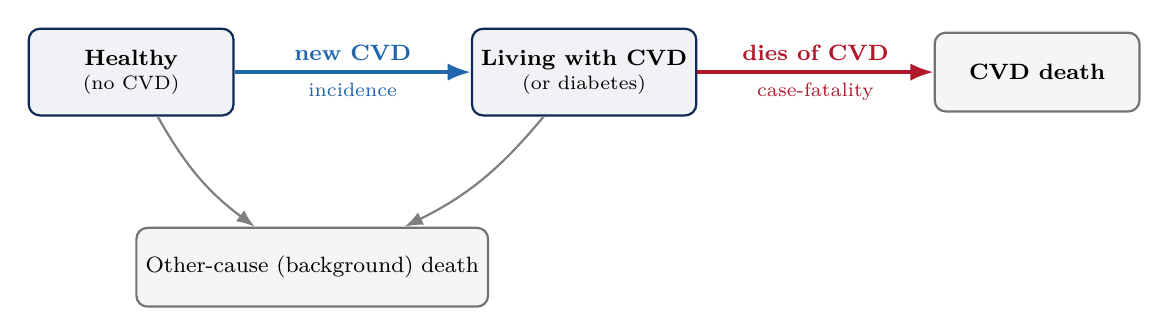
\begin{tikzpicture}[
   >=Latex, node distance = 16mm and 30mm, font=\footnotesize,
   state/.style = {rectangle, rounded corners, draw=wbnavy, thick, fill=wbnavy!6,
                   minimum width=26mm, minimum height=11mm, align=center},
   death/.style = {rectangle, rounded corners, draw=black!55, thick, fill=black!4,
                   minimum width=26mm, minimum height=10mm, align=center}]
  \node[state] (well) {\textbf{Healthy}\\[-1pt]\scriptsize (no CVD)};
  \node[state, right=of well] (sick) {\textbf{Living with CVD}\\[-1pt]\scriptsize (or diabetes)};
  \node[death, right=of sick] (cvd)  {\textbf{CVD death}};
  \node[death, below=14mm of well, xshift=23mm] (bg) {Other-cause (background) death};

  \draw[->, very thick, incidencecol]
       (well) -- node[above, midway, text=incidencecol]{\textbf{new CVD}}
                  node[below, midway, text=incidencecol, font=\scriptsize]{incidence} (sick);
  \draw[->, very thick, casefatalcol]
       (sick) -- node[above, midway, text=casefatalcol]{\textbf{dies of CVD}}
                  node[below, midway, text=casefatalcol, font=\scriptsize]{case-fatality} (cvd);
  \draw[->, thick, bgmortcol] (well) to[bend right=12] (bg);
  \draw[->, thick, bgmortcol] (sick) to[bend left=12]  (bg);
\end{tikzpicture}
\end{center}

\vspace{-2pt}
\begin{columns}[T]
\begin{column}{0.33\textwidth}\footnotesize
\textcolor{incidencecol}{\textbf{Fewer people fall ill}}\\ \scriptsize Primary prevention \& \emph{all} public-health policies lower \textbf{incidence}.
\end{column}
\begin{column}{0.34\textwidth}\footnotesize
\textcolor{casefatalcol}{\textbf{More people survive}}\\ \scriptsize Secondary prevention, treatment \& tobacco policy lower \textbf{case-fatality}.
\end{column}
\begin{column}{0.31\textwidth}\footnotesize
\textcolor{bgmortcol}{\textbf{Background mortality}}\\ \scriptsize Other-cause deaths from demography; unchanged by these interventions.
\end{column}
\end{columns}

\vspace{3pt}

\scriptsize No recovery/remission transition is modeled: people living
with CVD remain at elevated risk (a conservative assumption). Source:
model engine, \texttt{06\_run\_scenarios\_indonesia\_fair.R}.
\end{frame}

\section{The interventions}\label{the-interventions}

\begin{frame}{Clinical interventions (FAIR Choices)}
\phantomsection\label{clinical-interventions-fair-choices}
\begin{table}[!h]
\centering\begingroup\fontsize{8.5}{10.5}\selectfont

\begin{tabular}[t]{>{\raggedright\arraybackslash}p{4.6cm}>{\raggedright\arraybackslash}p{6.4cm}>{\raggedright\arraybackslash}p{3.0cm}}
\toprule
\textbf{Intervention} & \textbf{Target population} & \textbf{Model effect}\\
\midrule
\textbf{Primary CVD prevention} & Adults at cardiovascular risk & \textcolor{incidencecol}{Incidence}\\
\textbf{Type-2 diabetes treatment} & People with type-2 diabetes & \textcolor{casefatalcol}{Case-fatality}\\
\textbf{Heart-attack secondary prevention} & Heart-attack (IHD) survivors & \textcolor{casefatalcol}{Case-fatality}\\
\textbf{Stroke secondary prevention} & Stroke survivors & \textcolor{casefatalcol}{Case-fatality}\\
\textbf{Chronic \& acute heart-failure care} & Heart-failure patients & \textcolor{casefatalcol}{Case-fatality}\\
\addlinespace
\textbf{RHD secondary prevention \& surgery} & Rheumatic heart disease patients & \textcolor{casefatalcol}{Case-fatality}\\
\bottomrule
\end{tabular}
\endgroup{}
\end{table}

\vspace{2pt}

\footnotesize \textbf{Implementation scenario (all clinical interventions):}
coverage scales up \textbf{linearly from 31\% to 80\%} of the eligible
population between 2025 and 2050 (RHD surgery from a lower base). Effect
sizes are drawn from the FAIR Choices intervention taxonomy; primary
prevention lowers who develops CVD, while secondary prevention and
treatment improve survival. \scriptsize Source: workbook
\texttt{Selected\_Interventions}.
\end{frame}

\begin{frame}{Public-health interventions (fiscal \& regulatory policy)}
\phantomsection\label{public-health-interventions-fiscal-regulatory-policy}
\begin{table}[!h]
\centering\begingroup\fontsize{8}{10}\selectfont

\begin{tabular}[t]{>{\raggedright\arraybackslash}p{3.1cm}>{\raggedright\arraybackslash}p{2.4cm}>{\raggedright\arraybackslash}p{3.2cm}>{\raggedright\arraybackslash}p{5.0cm}}
\toprule
\textbf{Policy} & \textbf{Risk factor} & \textbf{Model effect} & \textbf{Implementation lever}\\
\midrule
\textbf{Tobacco tax} & Tobacco & \textcolor{incidencecol}{Incidence} + \textcolor{casefatalcol}{survival} & Raise tax to 75\% of retail price\\
\textbf{Tobacco policy package} & Tobacco & \textcolor{incidencecol}{Incidence} + \textcolor{casefatalcol}{survival} & Clean-air law, mass media, ad ban\\
\textbf{Sodium policy package} & Dietary salt/sodium & \textcolor{incidencecol}{Incidence} & Reformulation, labelling, media, procurement\\
\textbf{Trans-fat elimination} & Industrial trans-fat & \textcolor{incidencecol}{Incidence} & Best-practice industrial TFA ban\\
\textbf{Sugary-drink (SSB) tax} & Sugary drinks & \textcolor{incidencecol}{Incidence} & Price increase via excise\\
\addlinespace
\textbf{Alcohol tax / ad ban} & Alcohol & \textcolor{incidencecol}{Incidence} & Price increase; advertising ban\\
\bottomrule
\end{tabular}
\endgroup{}
\end{table}

\vspace{1pt}

\footnotesize Policies reduce exposure (smoking, salt, trans-fat,
sugary-drink and alcohol intake), lowering CVD \textbf{incidence}.
\textbf{Tobacco} policies additionally improve \textbf{survival} after
CVD. Packages are modeled as single joint runs of their component
measures. \scriptsize Source: workbook \texttt{Selected\_Interventions}
/ \texttt{Policy\_Levers}.
\end{frame}

\begin{frame}{Data sources}
\phantomsection\label{data-sources}
\begin{table}[!h]
\centering\begingroup\fontsize{7.4}{9.4}\selectfont

\begin{tabular}[t]{>{\raggedright\arraybackslash}p{3.4cm}>{\raggedright\arraybackslash}p{4.2cm}>{\raggedright\arraybackslash}p{2.0cm}>{\raggedright\arraybackslash}p{4.3cm}}
\toprule
\textbf{Model component} & \textbf{Primary source} & \textbf{Years / version} & \textbf{Use in model}\\
\midrule
\textbf{Population \& demography} & UN World Population Prospects & 2024 revision & Population, background mortality, life expectancy\\
\textbf{Cause-specific mortality \& disease rates} & GBD (Indonesia) & 2023 & Baseline burden \& calibration targets\\
\textbf{Disability weights (healthy-years lost)} & GBD & 2023 & DALYs\\
\textbf{Clinical intervention effects} & FAIR Choices intervention taxonomy & current & Incidence \& case-fatality effects\\
\textbf{Public-health effect sizes} & Published risk-factor evidence (in workbook) & current & Incidence \& survival effects\\
\addlinespace
\textbf{Intervention \& policy costs} & Programme \& policy unit costs (in workbook) & price year 2023 & Budget impact \& cost-effectiveness\\
\textbf{Economic valuation (VSL/VSLY)} & Reference Case guidance (Robinson 2019) & 2019 & Monetized benefits \& benefit--cost\\
\textbf{International 40q30 comparison} & WPP-scaled ASEAN comparison series & 1995--2050 & Benchmarking Indonesia vs.\ neighbours\\
\bottomrule
\end{tabular}
\endgroup{}
\end{table}

\vspace{1pt}

\scriptsize Sources verified in the modeling pipeline and input
workbooks. Specific effect-size and cost citations are documented in the
input workbooks. Population: UN World Population Prospects 2024; GBD
(GBD 2023 Cardiovascular Diseases and Risks Collaborators 2025;
Schumacher et al. 2024); economic valuation (Robinson, Hammitt, and
O'Keeffe 2019).
\end{frame}

\section{Health impact and value for
money}\label{health-impact-and-value-for-money}

\begin{frame}{Public health: impact by policy}
\phantomsection\label{public-health-impact-by-policy}
\begin{table}[!h]
\centering\begingroup\fontsize{8}{10}\selectfont

\begin{tabular}[t]{>{\raggedright\arraybackslash}p{4.6cm}rrrr}
\toprule
\textbf{Public-health policy} & \textbf{\makecell[c]{Deaths averted\\(cumulative)}} & \textbf{\makecell[c]{CVD 40q30\\2050}} & \textbf{\makecell[c]{40q30 reduction\\2050}} & \textbf{\makecell[c]{Deaths reduction\\2050}}\\
\midrule
\textbf{Tobacco tax} & 724,000 & 8.6\% & 5.2\% & 3.3\%\\
\textbf{Sodium policy package} & 540,000 & 8.7\% & 4.0\% & 3.0\%\\
\textbf{Tobacco policy package} & 435,000 & 8.8\% & 3.1\% & 2.0\%\\
\textbf{Mandatory sodium reformulation} & 294,000 & 8.9\% & 2.2\% & 1.6\%\\
\textbf{Tobacco mass-media campaign} & 178,000 & 9.0\% & 1.3\% & 0.8\%\\
\addlinespace
\textbf{Smoke-free / clean-air law} & 150,000 & 9.0\% & 1.1\% & 0.7\%\\
\textbf{Sodium front-of-pack labelling} & 148,000 & 9.0\% & 1.1\% & 0.8\%\\
\textbf{Tobacco advertising ban} & 109,000 & 9.0\% & 0.8\% & 0.5\%\\
\textbf{Supportive public-institution environment} & 104,000 & 9.0\% & 0.8\% & 0.6\%\\
\textbf{Sodium mass-media campaign} & 0 & 9.1\% & -0.0\% & -0.0\%\\
\addlinespace
\cellcolor[HTML]{E7F4F1}{\textbf{\textbf{All public health (combined)}}} & \cellcolor[HTML]{E7F4F1}{\textbf{1,649,000}} & \cellcolor[HTML]{E7F4F1}{\textbf{8.0\%}} & \cellcolor[HTML]{E7F4F1}{\textbf{11.9\%}} & \cellcolor[HTML]{E7F4F1}{\textbf{8.0\%}}\\
\bottomrule
\end{tabular}
\endgroup{}
\end{table}

\vspace{1pt}

\footnotesize Cumulative deaths averted over 2025--2050 vs.~the
status-quo baseline. Packages (tobacco, sodium) are single joint runs of
their component measures; individual sodium/tobacco measures are listed
in the appendix. \scriptsize Source: public-health cost/value workbook.
\end{frame}

\begin{frame}{Clinical: impact and cost-effectiveness}
\phantomsection\label{clinical-impact-and-cost-effectiveness}
\begin{table}[!h]
\centering\begingroup\fontsize{8}{10}\selectfont

\resizebox{\ifdim\width>\linewidth\linewidth\else\width\fi}{!}{
\begin{tabular}[t]{>{}lrrrrrr}
\toprule
\textbf{Clinical intervention} & \textbf{\makecell[c]{Deaths averted\\(cumulative)}} & \textbf{\makecell[c]{CVD 40q30\\2050}} & \textbf{\makecell[c]{40q30 red.\\2050}} & \textbf{\makecell[c]{Deaths red.\\2050}} & \textbf{\makecell[c]{Cost per\\death averted}} & \textbf{\makecell[c]{Annual cost\\per capita}}\\
\midrule
\textbf{Primary CVD prevention} & 1,322,000 & 7.6\% & 16.5\% & 10.9\% & US\$919 & US\$0.25\\
\textbf{Type-2 diabetes treatment} & 369,000 & 9.1\% & 0.3\% & 2.4\% & US\$26,411 & US\$1.97\\
\textbf{Heart-attack secondary prevention} & 141,000 & 8.9\% & 1.8\% & 0.8\% & US\$21,376 & US\$0.61\\
\textbf{Chronic heart-failure care} & 77,000 & 9.0\% & 0.9\% & 0.5\% & US\$7,831 & US\$0.13\\
\textbf{Acute heart-failure care} & 69,000 & 9.0\% & 0.6\% & 0.5\% & US\$13,210 & US\$0.19\\
\addlinespace
\textbf{Stroke secondary prevention} & 31,000 & 9.1\% & 0.3\% & 0.2\% & US\$56,216 & US\$0.36\\
\textbf{RHD secondary prevention} & 6,000 & 9.1\% & 0.0\% & 0.0\% & US\$24,755 & US\$0.03\\
\cellcolor[HTML]{EAF1FB}{\textbf{\textbf{All clinical (combined)}}} & \cellcolor[HTML]{EAF1FB}{\textbf{1,978,000}} & \cellcolor[HTML]{EAF1FB}{\textbf{7.3\%}} & \cellcolor[HTML]{EAF1FB}{\textbf{19.8\%}} & \cellcolor[HTML]{EAF1FB}{\textbf{14.9\%}} & \cellcolor[HTML]{EAF1FB}{\textbf{US\$8,312}} & \cellcolor[HTML]{EAF1FB}{\textbf{US\$3.33}}\\
\bottomrule
\end{tabular}}
\endgroup{}
\end{table}

\vspace{1pt}

\footnotesize Cost per death averted uses \textbf{discounted}
incremental cost (3\%/yr). Annual cost per capita = undiscounted
incremental cost averaged over 26 years and Indonesia's population.
Costs in market US\$ (price year 2023); perspective: health system.
\scriptsize Source: clinical cost/value workbook.
\end{frame}

\begin{frame}{Clinical: benefit--cost analysis}
\phantomsection\label{clinical-benefitcost-analysis}
\begin{table}[!h]
\centering\begingroup\fontsize{8}{10}\selectfont

\resizebox{\ifdim\width>\linewidth\linewidth\else\width\fi}{!}{
\begin{tabular}[t]{>{}lrrrrr}
\toprule
\textbf{Clinical intervention} & \textbf{Deaths averted} & \textbf{\makecell[c]{Cost per\\death averted}} & \textbf{Benefits (PV)} & \textbf{Net benefit (PV)} & \textbf{\makecell[c]{Benefit--cost\\ratio}}\\
\midrule
\textbf{Primary CVD prevention} & 1,322,000 & US\$919 & Int\$1.5T & Int\$1.5T & 418\\
\textbf{Type-2 diabetes treatment} & 369,000 & US\$26,411 & Int\$421.3B & Int\$392.0B & 14.4\\
\textbf{Heart-attack secondary prevention} & 141,000 & US\$21,376 & Int\$159.9B & Int\$150.8B & 17.7\\
\textbf{Chronic heart-failure care} & 77,000 & US\$7,831 & Int\$87.7B & Int\$85.9B & 48.4\\
\textbf{Acute heart-failure care} & 69,000 & US\$13,210 & Int\$78.2B & Int\$75.5B & 28.8\\
\addlinespace
\textbf{Stroke secondary prevention} & 31,000 & US\$56,216 & Int\$35.7B & Int\$30.4B & 6.7\\
\textbf{RHD secondary prevention} & 6,000 & US\$24,755 & Int\$6.9B & Int\$6.5B & 15.3\\
\cellcolor[HTML]{EAF1FB}{\textbf{\textbf{All clinical (combined)}}} & \cellcolor[HTML]{EAF1FB}{\textbf{1,978,000}} & \cellcolor[HTML]{EAF1FB}{\textbf{US\$8,312}} & \cellcolor[HTML]{EAF1FB}{\textbf{Int\$2.3T}} & \cellcolor[HTML]{EAF1FB}{\textbf{Int\$2.2T}} & \cellcolor[HTML]{EAF1FB}{\textbf{46.0}}\\
\bottomrule
\end{tabular}}
\endgroup{}
\end{table}

\vspace{1pt}

\footnotesize Benefits = value of averted mortality (preferred VSL,
income elasticity 1.5), in PPP international dollars, base year 2025,
discounted at 3\%/yr; standing: societal; scope: partial (mortality
benefit only). A ratio above 1 means benefits exceed costs.
\scriptsize Source: clinical cost/value workbook, preferred-VSL case.
\end{frame}

\begin{frame}{Public health: cost-effectiveness}
\phantomsection\label{public-health-cost-effectiveness}
\begin{table}[!h]
\centering\begingroup\fontsize{8}{10}\selectfont

\resizebox{\ifdim\width>\linewidth\linewidth\else\width\fi}{!}{
\begin{tabular}[t]{>{}lrrrrrr}
\toprule
\textbf{Public-health policy} & \textbf{\makecell[c]{Deaths averted\\(cumulative)}} & \textbf{\makecell[c]{CVD 40q30\\2050}} & \textbf{\makecell[c]{40q30 red.\\2050}} & \textbf{\makecell[c]{Deaths red.\\2050}} & \textbf{\makecell[c]{Cost per\\death averted}} & \textbf{\makecell[c]{Annual cost\\per capita}}\\
\midrule
\textbf{Tobacco tax} & 724,000 & 8.6\% & 5.2\% & 3.3\% & US\$283 & US\$0.04\\
\textbf{Sodium policy package} & 540,000 & 8.7\% & 4.0\% & 3.0\% & US\$333 & US\$0.03\\
\textbf{Tobacco policy package} & 435,000 & 8.8\% & 3.1\% & 2.0\% & US\$272 & US\$0.02\\
\textbf{Mandatory sodium reformulation} & 294,000 & 8.9\% & 2.2\% & 1.6\% & US\$153 & US\$0.01\\
\textbf{Tobacco mass-media campaign} & 178,000 & 9.0\% & 1.3\% & 0.8\% & US\$222 & US\$0.01\\
\addlinespace
\textbf{Smoke-free / clean-air law} & 150,000 & 9.0\% & 1.1\% & 0.7\% & US\$262 & US\$0.01\\
\textbf{Sodium front-of-pack labelling} & 148,000 & 9.0\% & 1.1\% & 0.8\% & US\$303 & US\$0.01\\
\textbf{Tobacco advertising ban} & 109,000 & 9.0\% & 0.8\% & 0.5\% & US\$361 & US\$0.01\\
\textbf{Supportive public-institution environment} & 104,000 & 9.0\% & 0.8\% & 0.6\% & US\$433 & US\$0.01\\
\textbf{Sodium mass-media campaign} & 0 & 9.1\% & -0.0\% & -0.0\% & US\$NA & US\$0.01\\
\addlinespace
\cellcolor[HTML]{E7F4F1}{\textbf{\textbf{All public health (combined)}}} & \cellcolor[HTML]{E7F4F1}{\textbf{1,649,000}} & \cellcolor[HTML]{E7F4F1}{\textbf{8.0\%}} & \cellcolor[HTML]{E7F4F1}{\textbf{11.9\%}} & \cellcolor[HTML]{E7F4F1}{\textbf{8.0\%}} & \cellcolor[HTML]{E7F4F1}{\textbf{US\$305}} & \cellcolor[HTML]{E7F4F1}{\textbf{US\$0.09}}\\
\bottomrule
\end{tabular}}
\endgroup{}
\end{table}

\vspace{1pt}

\footnotesize Fiscal and regulatory policies reach the whole population
at very low per-person cost, so cost per death averted is far lower than
for clinical care. Same costing conventions as the clinical table.
\scriptsize Source: public-health cost/value workbook.
\end{frame}

\begin{frame}{Public health: benefit--cost analysis}
\phantomsection\label{public-health-benefitcost-analysis}
\begin{table}[!h]
\centering\begingroup\fontsize{8}{10}\selectfont

\resizebox{\ifdim\width>\linewidth\linewidth\else\width\fi}{!}{
\begin{tabular}[t]{>{}lrrrrr}
\toprule
\textbf{Public-health policy} & \textbf{Deaths averted} & \textbf{\makecell[c]{Cost per\\death averted}} & \textbf{Benefits (PV)} & \textbf{Net benefit (PV)} & \textbf{\makecell[c]{Benefit--cost\\ratio}}\\
\midrule
\textbf{Tobacco tax} & 724,000 & US\$283 & Int\$819.8B & Int\$819.2B & 1,330\\
\textbf{Sodium policy package} & 540,000 & US\$333 & Int\$616.8B & Int\$616.3B & 1,140\\
\textbf{Tobacco policy package} & 435,000 & US\$272 & Int\$492.0B & Int\$491.6B & 1,390\\
\textbf{Mandatory sodium reformulation} & 294,000 & US\$153 & Int\$336.5B & Int\$336.3B & 2,500\\
\textbf{Tobacco mass-media campaign} & 178,000 & US\$222 & Int\$201.2B & Int\$201.1B & 1,700\\
\addlinespace
\textbf{Smoke-free / clean-air law} & 150,000 & US\$262 & Int\$170.1B & Int\$170.0B & 1,440\\
\textbf{Sodium front-of-pack labelling} & 148,000 & US\$303 & Int\$169.1B & Int\$169.0B & 1,260\\
\textbf{Tobacco advertising ban} & 109,000 & US\$361 & Int\$123.6B & Int\$123.5B & 1,050\\
\textbf{Supportive public-institution environment} & 104,000 & US\$433 & Int\$118.6B & Int\$118.5B & 880\\
\textbf{Sodium mass-media campaign} & 0 & US\$NA & Int\$0.0 & Int\$-134.7M & -0.0\\
\addlinespace
\cellcolor[HTML]{E7F4F1}{\textbf{\textbf{All public health (combined)}}} & \cellcolor[HTML]{E7F4F1}{\textbf{1,649,000}} & \cellcolor[HTML]{E7F4F1}{\textbf{US\$305}} & \cellcolor[HTML]{E7F4F1}{\textbf{Int\$1.9T}} & \cellcolor[HTML]{E7F4F1}{\textbf{Int\$1.9T}} & \cellcolor[HTML]{E7F4F1}{\textbf{1,240}}\\
\bottomrule
\end{tabular}}
\endgroup{}
\end{table}

\vspace{1pt}

\footnotesize Because fiscal/regulatory policies cost little to
implement relative to the mortality they avert, their benefit--cost
ratios are very large. Same valuation conventions (preferred VSL, PPP
international dollars, base year 2025, 3\%/yr) as the clinical BCA.
\scriptsize Source: public-health cost/value workbook.
\end{frame}

\section{The combined package}\label{the-combined-package}

\begin{frame}{Clinical + public health: better together}
\phantomsection\label{clinical-public-health-better-together}
\begin{table}[!h]
\centering\begingroup\fontsize{8.5}{10.5}\selectfont

\resizebox{\ifdim\width>\linewidth\linewidth\else\width\fi}{!}{
\begin{tabular}[t]{>{}lrrrrrr}
\toprule
\textbf{Package} & \textbf{\makecell[c]{Deaths averted\\(cumulative)}} & \textbf{\makecell[c]{40q30 red.\\2050}} & \textbf{\makecell[c]{CVD 40q30\\2050}} & \textbf{\makecell[c]{Total cost\\(PV)}} & \textbf{\makecell[c]{Cost per\\death averted}} & \textbf{\makecell[c]{Benefit--cost\\ratio}}\\
\midrule
\textbf{All clinical (combined)} & 1,978,000 & 19.8\% & 7.3\% & US\$16.4B & US\$8,312 & 46.0\\
\textbf{All public health (combined)} & 1,649,000 & 11.9\% & 8.0\% & US\$503.2M & US\$305 & 1,240\\
\cellcolor[HTML]{FCEFCB}{\textbf{\textbf{Clinical + public health (combined)}}} & \cellcolor[HTML]{FCEFCB}{\textbf{3,453,000}} & \cellcolor[HTML]{FCEFCB}{\textbf{29.2\%}} & \cellcolor[HTML]{FCEFCB}{\textbf{6.4\%}} & \cellcolor[HTML]{FCEFCB}{\textbf{US\$16.6B}} & \cellcolor[HTML]{FCEFCB}{\textbf{US\$4,814}} & \cellcolor[HTML]{FCEFCB}{\textbf{79.1}}\\
\bottomrule
\end{tabular}}
\endgroup{}
\end{table}

\vspace{2pt}
\begin{combinedblock}{The combined package is modeled as one run --- not a sum}
\footnotesize Because clinical and public-health effects overlap, the joint scenario is projected in a single run.
It averts about \textbf{3.5M deaths}, brings the 2050 CVD 40q30 down to
\textbf{6.4\%} (from 9.1\% at baseline), and yields a benefit--cost ratio of about
\textbf{79.1} --- a net benefit of roughly \textbf{Int\$3.9T}.
\end{combinedblock}
\end{frame}

\begin{frame}{CVD premature mortality: trajectory and neighbours}
\phantomsection\label{cvd-premature-mortality-trajectory-and-neighbours}
\begin{center}\includegraphics[width=\linewidth]{executive_slides_v1_files/figure-beamer/fig-40q30-1} \end{center}
\end{frame}

\section{What it means for Indonesia}\label{what-it-means-for-indonesia}

\begin{frame}{Policy implications}
\phantomsection\label{policy-implications}
\begin{columns}[T]
\begin{column}{0.5\textwidth}
\begin{itemize}\footnotesize\itemsep4pt
  \item \textbf{Biggest health gains come from doing both.} The combined package averts far more (\textasciitilde3.5M) than either family alone.
  \item \textbf{Public-health policies are exceptional value.} Population-wide fiscal/regulatory measures avert deaths at a fraction of clinical cost (ratios in the thousands).
  \item \textbf{Clinical scale-up delivers large, durable gains} in survival and premature mortality, at conventional cost-effectiveness.
\end{itemize}
\end{column}
\begin{column}{0.5\textwidth}
\begin{itemize}\footnotesize\itemsep4pt
  \item \textbf{Sequence for early wins.} Tobacco taxation and other prevention policies can start cutting risk quickly and cheaply, while clinical capacity scales up.
  \item \textbf{The 40q30 target is within reach.} The combined package bends Indonesia's premature-CVD-mortality curve down by about 29\% by 2050.
\end{itemize}
\end{column}
\end{columns}

\vspace{2pt}

\footnotesize These are model findings; translating them into policy
requires judgement on feasibility, financing and delivery. Model results
quantify the \emph{potential}; they are not a delivery guarantee.
\end{frame}

\begin{frame}{Limitations}
\phantomsection\label{limitations}
\begin{itemize}\footnotesize\itemsep3pt
  \item Results depend on \textbf{modeled epidemiological estimates} (GBD) and calibration; real burden may differ.
  \item \textbf{Effect sizes, future coverage, and unit costs are uncertain}; interventions are assumed to reach and sustain their targets.
  \item The disease model is \textbf{simplified} (healthy $\to$ living-with-CVD $\to$ death; no remission; no comorbidity interactions).
  \item Economic returns value \textbf{averted mortality only} (a partial benefit-cost scope) --- morbidity, productivity and downstream cost offsets are omitted, so returns are, if anything, understated.
  \item Projections are \textbf{scenarios, not forecasts or guarantees}; they show what is achievable if interventions are delivered as modeled.
\end{itemize}
\end{frame}

\begin{frame}{Three things to remember}
\phantomsection\label{three-things-to-remember}
\begin{columns}[T]
\begin{column}{0.33\textwidth}
\begin{combinedblock}{1. Both, together}
\footnotesize Clinical + public health averts \textbf{\textasciitilde3.5M deaths} by 2050 --- more than either alone.
\end{combinedblock}
\end{column}
\begin{column}{0.33\textwidth}
\begin{phblock}{2. Prevention pays}
\footnotesize Population policies return on the order of \textbf{1,240\texttimes} their cost.
\end{phblock}
\end{column}
\begin{column}{0.33\textwidth}
\begin{clinicalblock}{3. A reachable target}
\footnotesize Premature CVD mortality (40q30) falls \textbf{29\%} by 2050 under the combined package.
\end{clinicalblock}
\end{column}
\end{columns}

\vspace{4pt}
\begin{center}
\large Combined action against CVD could avert about \hlkey{3.5M deaths} and return about
\hlkey{79.1 int\$ per int\$ invested} through 2050.
\end{center}
\end{frame}

\section{Technical appendix}\label{technical-appendix}

\begin{frame}{Appendix 1 --- Scenario crosswalk}
\phantomsection\label{appendix-1-scenario-crosswalk}
\begin{table}[!h]
\centering\begingroup\fontsize{6}{8}\selectfont

\resizebox{\ifdim\width>\linewidth\linewidth\else\width\fi}{!}{
\begin{tabular}[t]{>{}l>{}ll}
\toprule
\textbf{Family} & \textbf{Workbook scenario id} & \textbf{Executive label}\\
\midrule
\textbf{Clinical (FAIR Choices)} & \ttfamily{I\\_CVD\\_PRIMARY} & Primary CVD prevention\\
\textbf{} & \ttfamily{I\\_T2D\\_TREATMENT} & Type-2 diabetes treatment\\
\textbf{} & \ttfamily{I\\_IHD\\_SECONDARY} & Heart-attack secondary prevention\\
\textbf{} & \ttfamily{I\\_HF\\_CHRONIC} & Chronic heart-failure care\\
\textbf{} & \ttfamily{I\\_HF\\_ACUTE} & Acute heart-failure care\\
\addlinespace
\textbf{} & \ttfamily{I\\_STROKE\\_SECONDARY} & Stroke secondary prevention\\
\textbf{} & \ttfamily{I\\_RHD\\_SECONDARY} & RHD secondary prevention\\
\textbf{} & \ttfamily{all} & All clinical (combined)\\
\textbf{Public health} & \ttfamily{I\\_PH\\_TOBACCO\\_TAX} & Tobacco tax\\
\textbf{} & \ttfamily{I\\_PH\\_SALT\\_POLICY} & Sodium policy package\\
\addlinespace
\textbf{} & \ttfamily{I\\_PH\\_TOBACCO\\_POLICY} & Tobacco policy package\\
\textbf{} & \ttfamily{I\\_PH\\_SALT\\_REFORM} & Mandatory sodium reformulation\\
\textbf{} & \ttfamily{I\\_PH\\_TOB\\_MEDIA} & Tobacco mass-media campaign\\
\textbf{} & \ttfamily{I\\_PH\\_TOB\\_CLEAN\\_AIR} & Smoke-free / clean-air law\\
\textbf{} & \ttfamily{I\\_PH\\_SALT\\_FOPL} & Sodium front-of-pack labelling\\
\addlinespace
\textbf{} & \ttfamily{I\\_PH\\_TOB\\_AD\\_BAN} & Tobacco advertising ban\\
\textbf{} & \ttfamily{I\\_PH\\_SALT\\_ENV} & Supportive public-institution environment\\
\textbf{} & \ttfamily{I\\_PH\\_SALT\\_MEDIA} & Sodium mass-media campaign\\
\textbf{} & \ttfamily{all\\_public\\_health} & All public health (combined)\\
\textbf{Combined} & \ttfamily{all\\_clinical\\_public\\_health} & Clinical + public health (combined)\\
\bottomrule
\end{tabular}}
\endgroup{}
\end{table}

\vspace{1pt}

\tiny Packages are single joint runs of their child measures (shown in
parentheses); child measures are omitted from the main tables to avoid
double-counting.
\end{frame}

\begin{frame}{Appendix 2 --- Definitions, horizons and assumptions}
\phantomsection\label{appendix-2-definitions-horizons-and-assumptions}
\footnotesize
\begin{columns}[T]
\begin{column}{0.5\textwidth}
\textbf{Metrics}
\begin{itemize}\scriptsize\itemsep2pt
  \item \textbf{Deaths averted (cumulative)} $=\sum_{t=2025}^{2050}(\text{baseline deaths}_t-\text{scenario deaths}_t)$, across modeled CVD \& diabetes causes.
  \item \textbf{\% reduction in deaths, 2050} $=100\times(\text{baseline}-\text{scenario})/\text{baseline}$ in 2050.
  \item \textbf{CVD 40q30} = probability of dying of CVD between exact ages 30 and 70 (six CVD causes, both sexes, single-year life table).
  \item \textbf{\% reduction in 40q30, 2050}: analogous to deaths.
\end{itemize}
\end{column}
\begin{column}{0.5\textwidth}
\textbf{Costing \& valuation}
\begin{itemize}\scriptsize\itemsep2pt
  \item Horizon 2025--2050; discount rate 3\%/yr; base year 2025; price year 2023.
  \item Costs in market US\$; cost perspective: health system.
  \item Benefits: averted-mortality value, \textbf{preferred VSL} (income elasticity 1.5), in PPP international dollars; standing societal; scope: partial mortality benefit.
  \item \textbf{Cost per death averted} uses discounted incremental cost.
\end{itemize}
\end{column}
\end{columns}

\vspace{3pt}

\scriptsize \textbf{Model.} Discrete-time state-transition model;
single-year ages 0--95; six CVD causes (IHD, ischemic stroke,
intracerebral haemorrhage, hypertensive heart disease, rheumatic heart
disease, cardiomyopathy \& myocarditis) plus type-2 diabetes; calibrated
to GBD 2023 (Nelder--Mead); demography and life expectancy from UN WPP
2024. \textbf{Validation:} Baseline reconciled across all three
workbooks (2050 deaths agree to 0.0000\%; 2050 CVD 40q30 to 0.0000\%).
All economic values were recalculated live from the formula workbooks.
\end{frame}

\begin{frame}{Appendix 3 --- References}
\phantomsection\label{appendix-3-references}
\scriptsize

\phantomsection\label{refs}
\begin{CSLReferences}{1}{0}
\bibitem[\citeproctext]{ref-GBDCVD2025}
GBD 2023 Cardiovascular Diseases and Risks Collaborators. 2025.
{``Global, Regional, and National Burden of Cardiovascular Diseases and
Risk Factors in 204 Countries and Territories, 1990--2023.''}
\emph{Journal of the American College of Cardiology} 86 (22):
2167--2243.

\bibitem[\citeproctext]{ref-Robinson2019VSL}
Robinson, Lisa A., James K. Hammitt, and Lucy O'Keeffe. 2019. {``Valuing
Mortality Risk Reductions in Global Benefit-Cost Analysis.''}
\emph{Journal of Benefit-Cost Analysis} 10 (S1): 15--50.
\url{https://doi.org/10.1017/bca.2018.26}.

\bibitem[\citeproctext]{ref-Schumacher2024GBD2021}
Schumacher, Austin E., Hmwe Hmwe Kyu, Catherine M. Antony, Aleksandr Y.
Aravkin, and Gulrez. 2024. {``Global Age-Sex-Specific Mortality, Life
Expectancy, and Population Estimates in 204 Countries and Territories
and 811 Subnational Locations, 1950--2021, and the Impact of the
COVID-19 Pandemic: A Comprehensive Demographic Analysis for the Global
Burden of Disease Study 2021.''} \emph{The Lancet} 403 (May):
1989--2056.
\url{https://doi.org/10.1016/S0140-6736(24)00476-8/ATTACHMENT/B6671C4E-CF06-47EB-AC9B-6A42B327599D/MMC3.PDF}.

\end{CSLReferences}
\end{frame}

\end{document}
